\documentclass[11pt]{article}

\usepackage{amsmath}
\usepackage{textcomp}
\usepackage[top=0.8in, bottom=0.8in, left=0.8in, right=0.8in]{geometry}
% Add other packages here %
\usepackage{subcaption}
\usepackage{float}
\usepackage{wrapfig}
\usepackage{graphicx}


% Put your group number and names in the author field %
\title{\bf Excercise 1.\\ Implementing a first Application in RePast: A Rabbits Grass Simulation.}
\author{Group \textnumero 10: Cosmin-Ionut Rusu, Sorin-Sebastian Mircea}

\begin{document}
\maketitle

\section{Implementation}
We followed the provided tutorial which served as a base for our implementation.

Grass is coded with green, and the rabbits are coded with blue.
\begin{figure}[H]
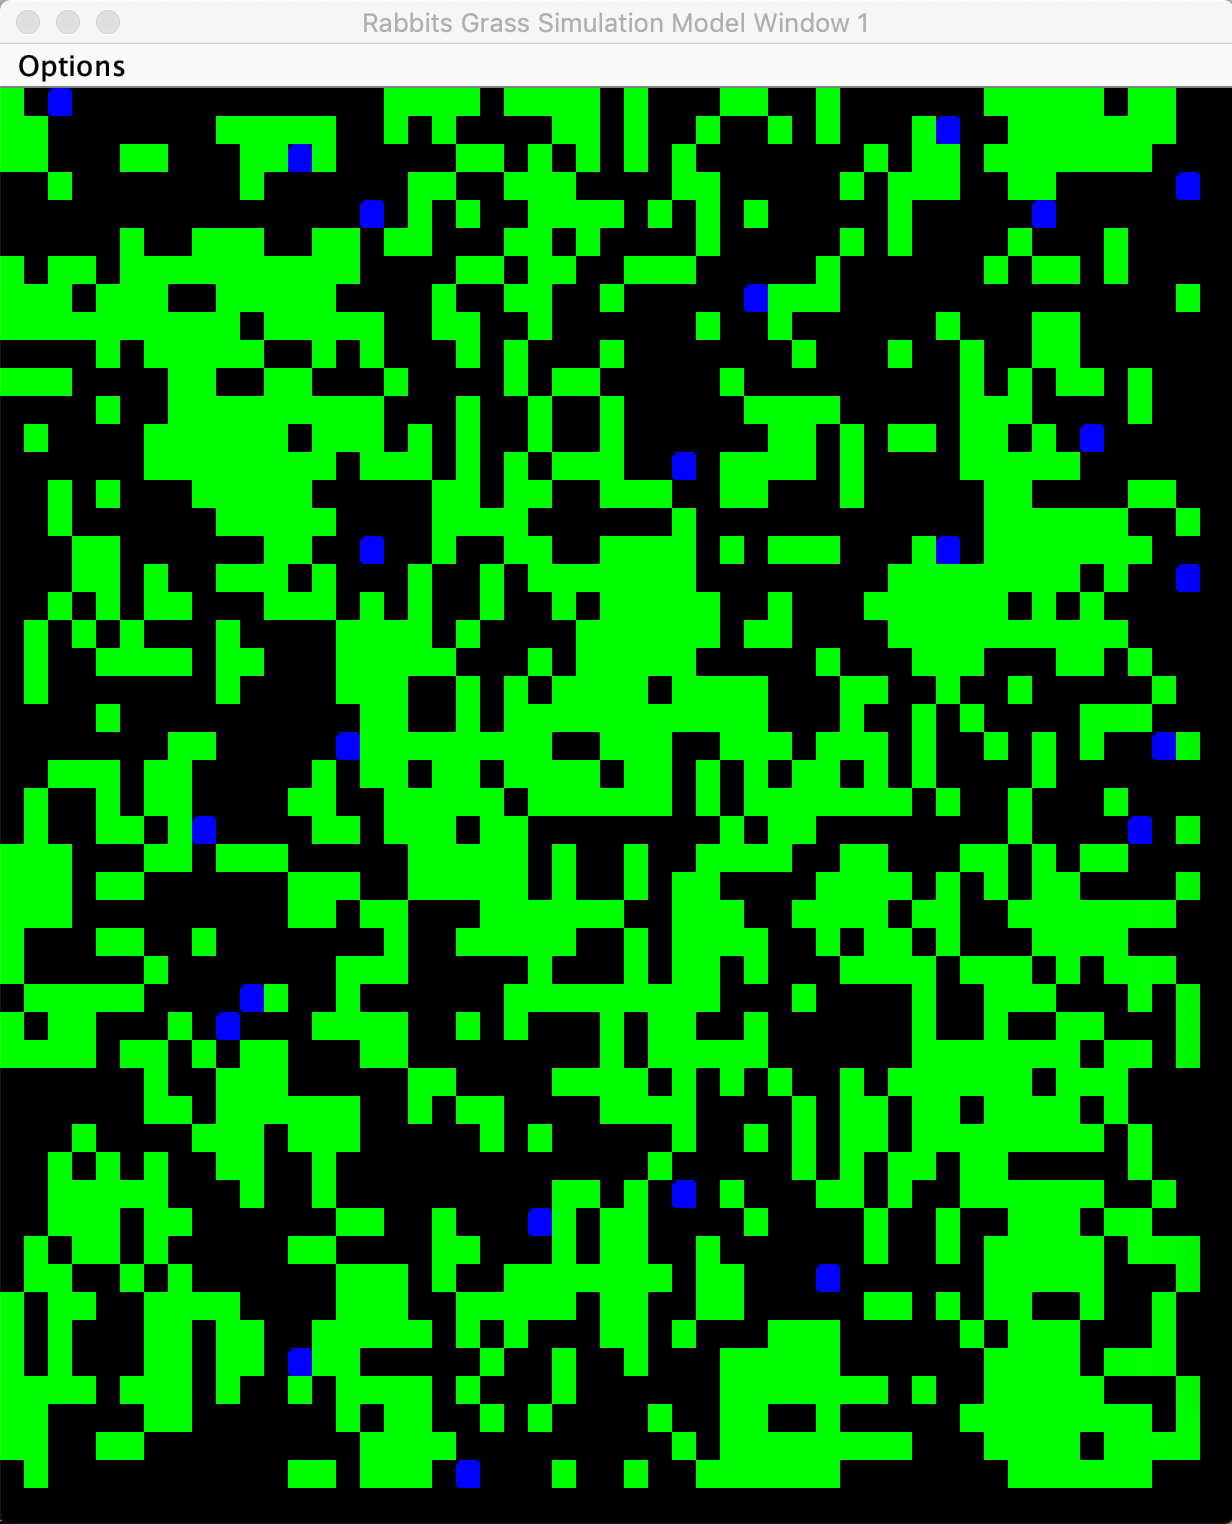
\includegraphics[width=0.59\textwidth]{world}
\centering
\label{fig:world}
\caption{Simulation world }
\end{figure}


\subsection*{Charts}
In order to better visualise the world we have created two charts:

\begin{enumerate}
\item  Showing the raport between the tiles of grass available in the world and the population of rabbits. The rabbit population is multiplied by a constant (in our case 100) in order to better depict the variations in population.
\begin{figure}[H]
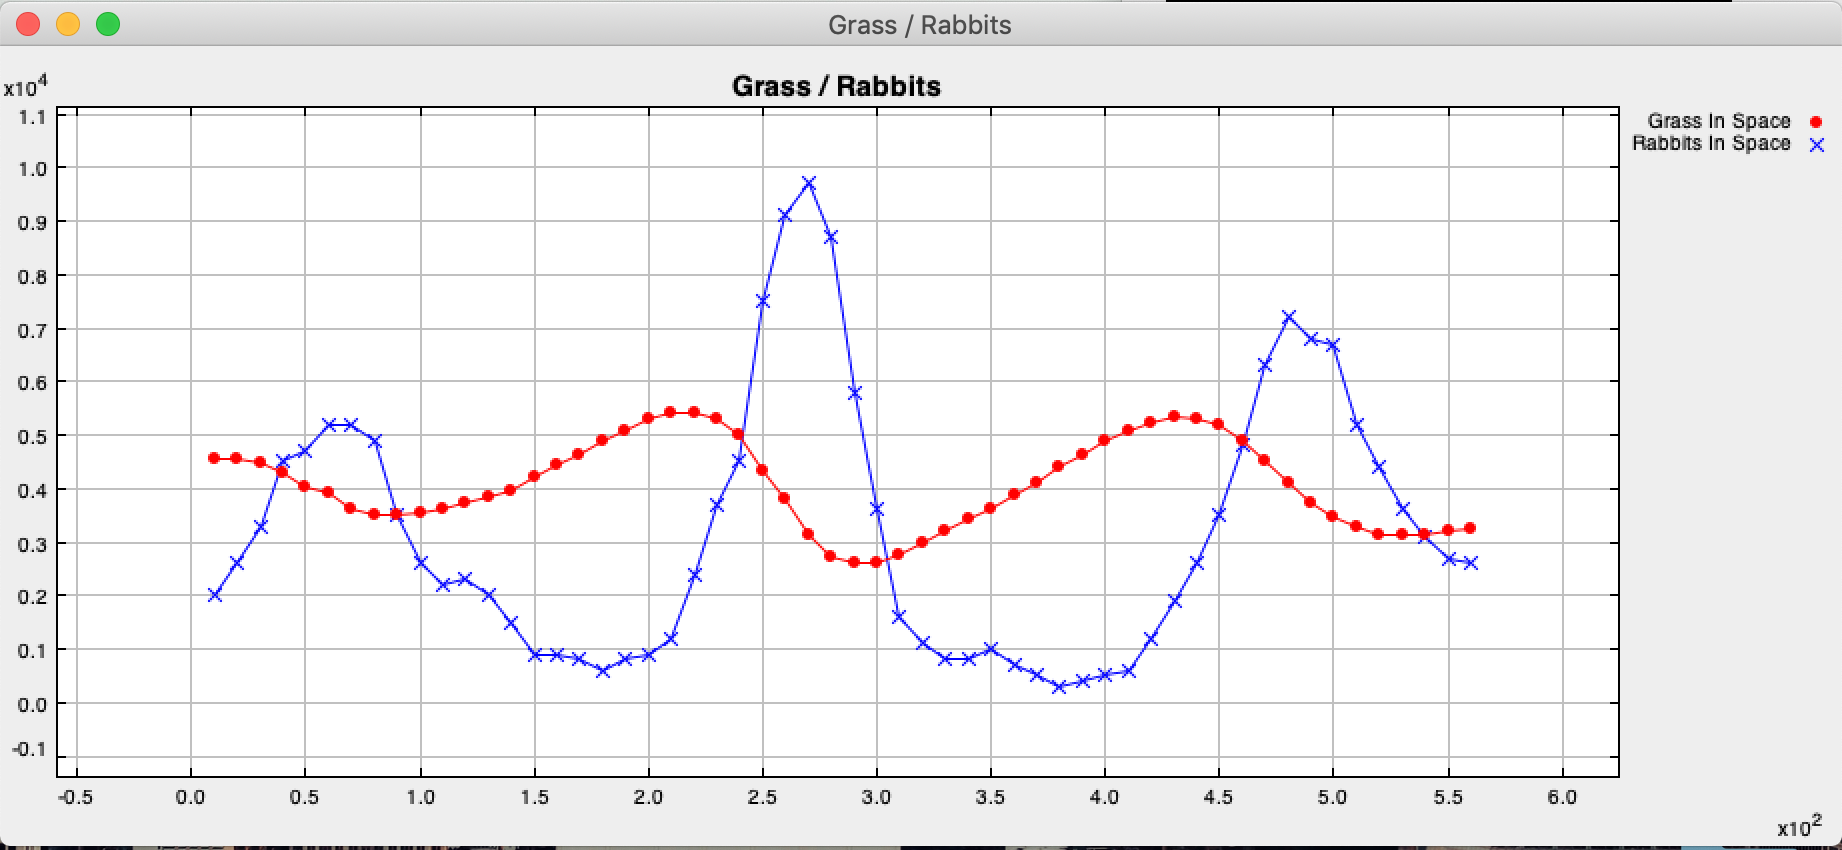
\includegraphics[width=0.59\textwidth]{chart}
\centering
\label{fig:grass-rabits-chart}
\caption{ Grass / Rabbits rapport }
\end{figure}

\item  Histogram of the rabbits energy at the current step
\begin{figure}[H]
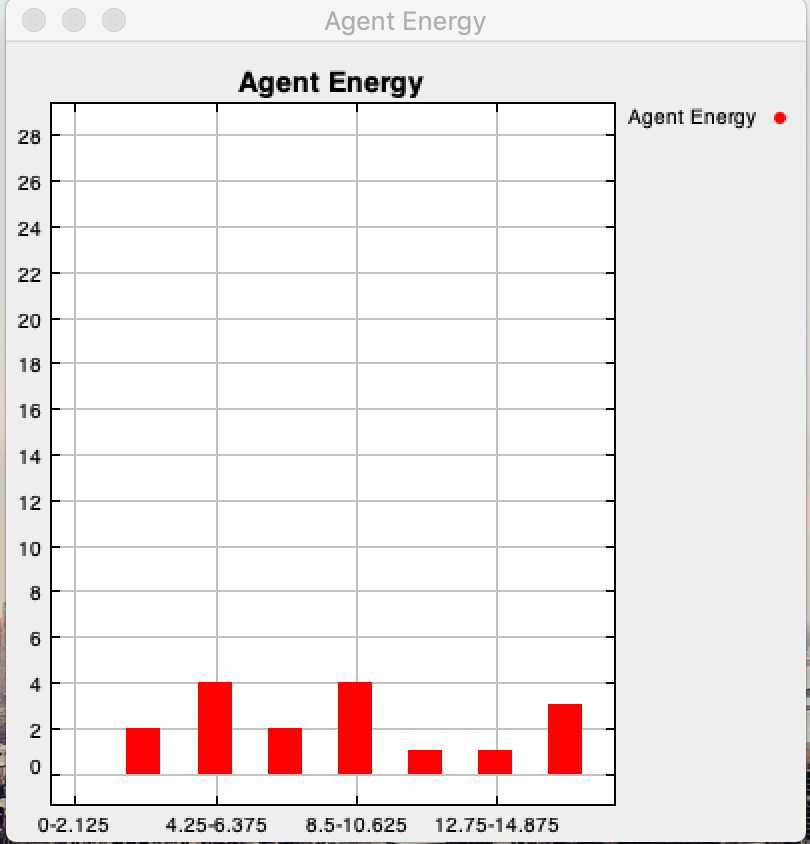
\includegraphics[width=0.59\textwidth]{histogram}
\centering
\label{fig:grass-rabits-histogram}
\caption{ Rabbits energy histogram }
\end{figure}

\end{enumerate}

\subsection*{Extra parameters}
We considered that the the the following parameters would need to be added (besides the already provided ones) in order to have a better control of the world:

\begin{itemize}
\item \textbf{EnergyLostByReproduction} - the energy that a rabbit is going to loose in order to reproduce (once it reaches the reproduction threshold)
\item \textbf{MinRabbitInitEnergy} and \textbf{MaxRabbitInitEnergy} - a range depicting the initial energy value of a rabbit; if the range is bigger than one, rabbits are randomly going to receive a value from the interval 
\end{itemize}






\subsection{Assumptions}
% Describe the assumptions of your world model and implementation (e.g. is the grass amount bounded in each cell) %

\subsection* {Action order}
The order in which our world is going to execute the possible actions can have an impact on the outcome (even this is negligible). Arbitrarily we chose the following order (that is executing during one step):
\begin{enumerate}
\item  Move agents
\item  Agents eat (if they are on a grass)
\item  Agents loose energy
\item  Agents give birth (if energy >= birthThreshold)
\item  Agents die (if energy = 0)
\item  New grass tiles are spawned
\end{enumerate}

\subsection* {Grass spawning}
We had to decide if we were going to spawn the grass only on the tiles that are unoccupied by the rabbits, or randomly everywhere. We chose the second one, when this happens the rabbits are instantly going to benefit by the extra food. The reason behind this was mainly due to the implementation reasons.

\subsection* {Initial energy levels}
This is a fair assumption since if a rabbit were to be born with an energy level >= birthThreshold, then it might reproduce right away and we will have more rabbits on the space.

\subsection* {Rabbit in impossibility of movement}
In the case that a rabbit cannot move due to it being surrounded by other rabbits, we chose for the rabbit to stay on place but still loose energy (as a penalty for not being able to search for food).

\subsection* {Collision system}
Rabbits cannot collide with other rabbits (during spawning and movement), it can move onto a grass tile (though, at that moment the grass will be consumed).

\subsection{Implementation Remarks}
Grass tiles cannot collide with other grass tiles (during spawning). Grass can be spawned on top of a rabbit but it will be consumed instantly by the rabbit.

\subsection* {Movements}

\begin{figure}[H]
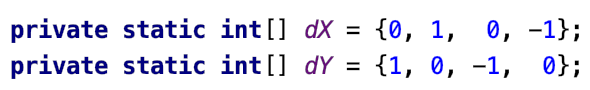
\includegraphics[width=0.59\textwidth]{rabbit-movement-1}
\centering
\label{fig:movement-directions}
\caption{ Directions of movement (Right, Down, Left, Up) }
\end{figure}

\begin{figure}[H]
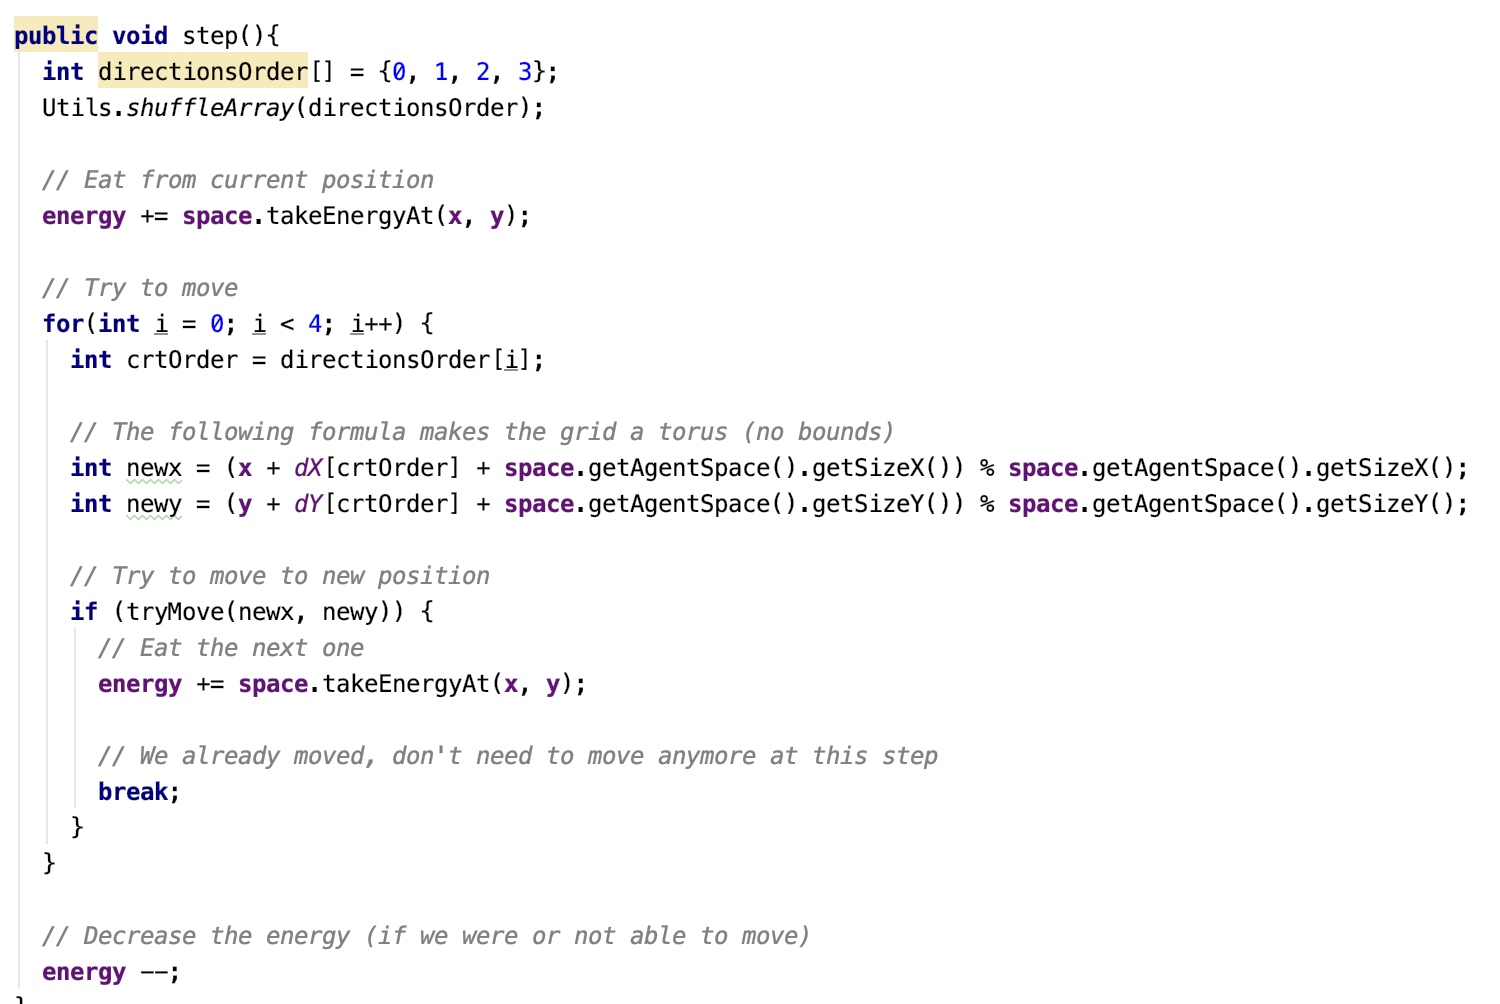
\includegraphics[width=1.0\textwidth]{rabbit-movement-2}
\centering
\label{fig:movement-directions}
\caption{ Rabbit procedure of doing one step }
\end{figure}




% Provide important details about your implementation, such as handling of boundary conditions %

\section{Results}
% In this section, you study and describe how different variables (e.g. birth threshold, grass growth rate etc.) or combinations of variables influence the results. Different experiments with diffrent settings are described below with your observations and analysis

\subsection{Experiment 1 ~ variating amount of initial rabbit (~500 ticks)}

\begin{figure}[H]
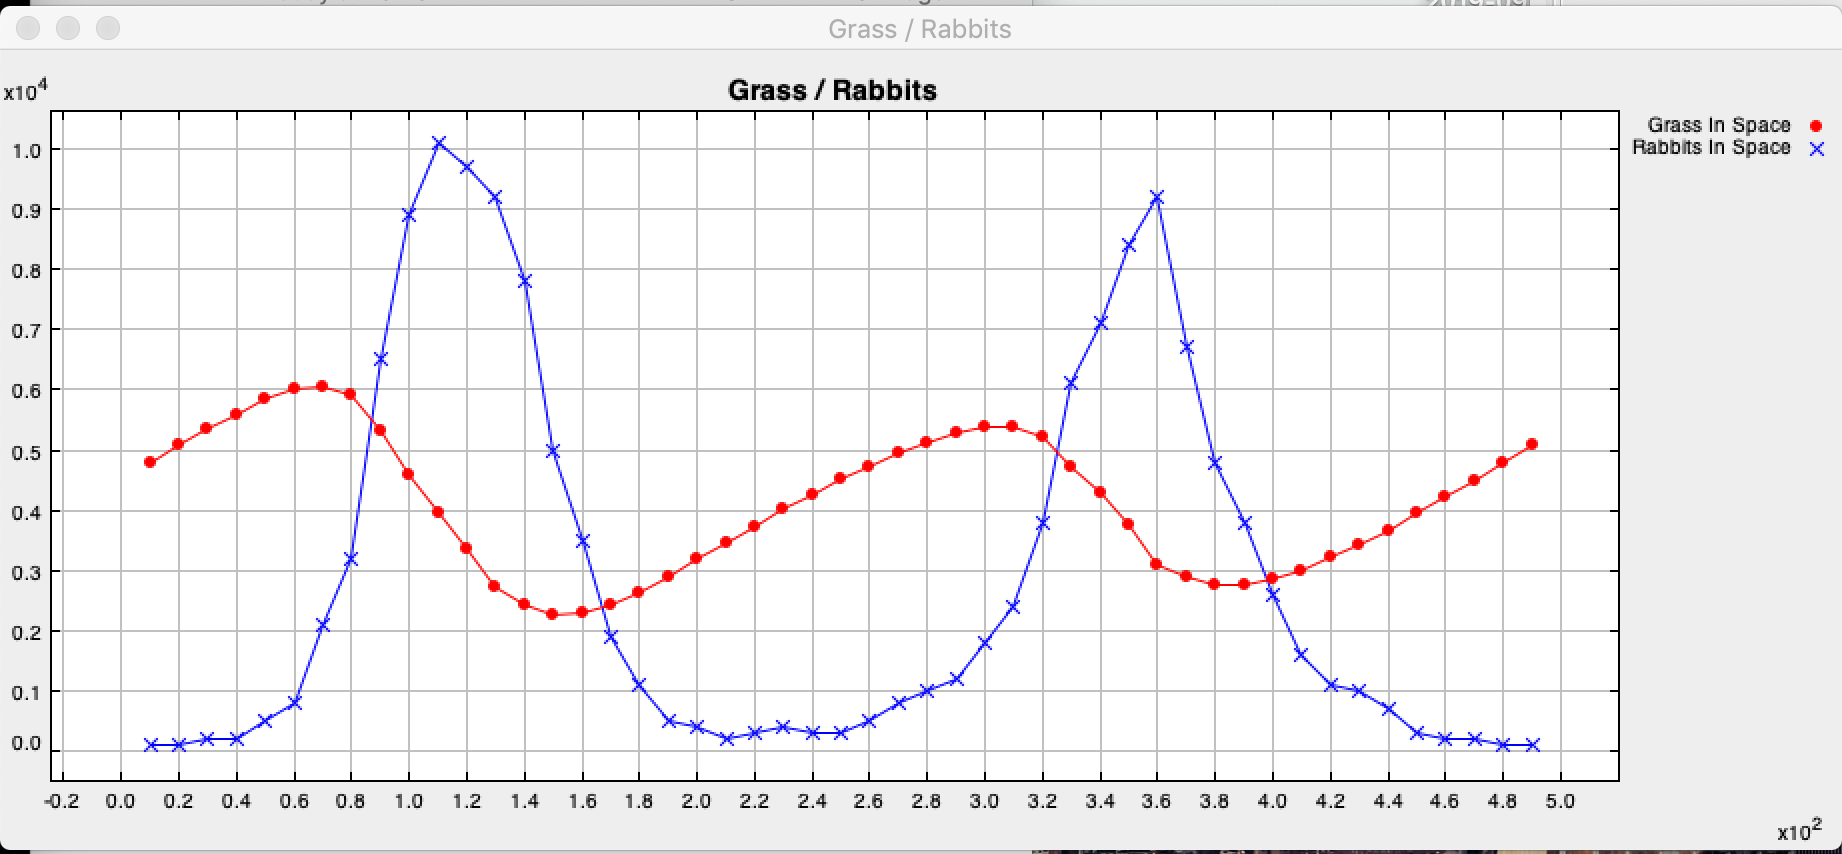
\includegraphics[width=1.0\textwidth]{ex1-chart-1}
\centering
\label{fig:ex1-1}
\caption{ 1 initial rabbit }
\end{figure}

\begin{figure}[H]
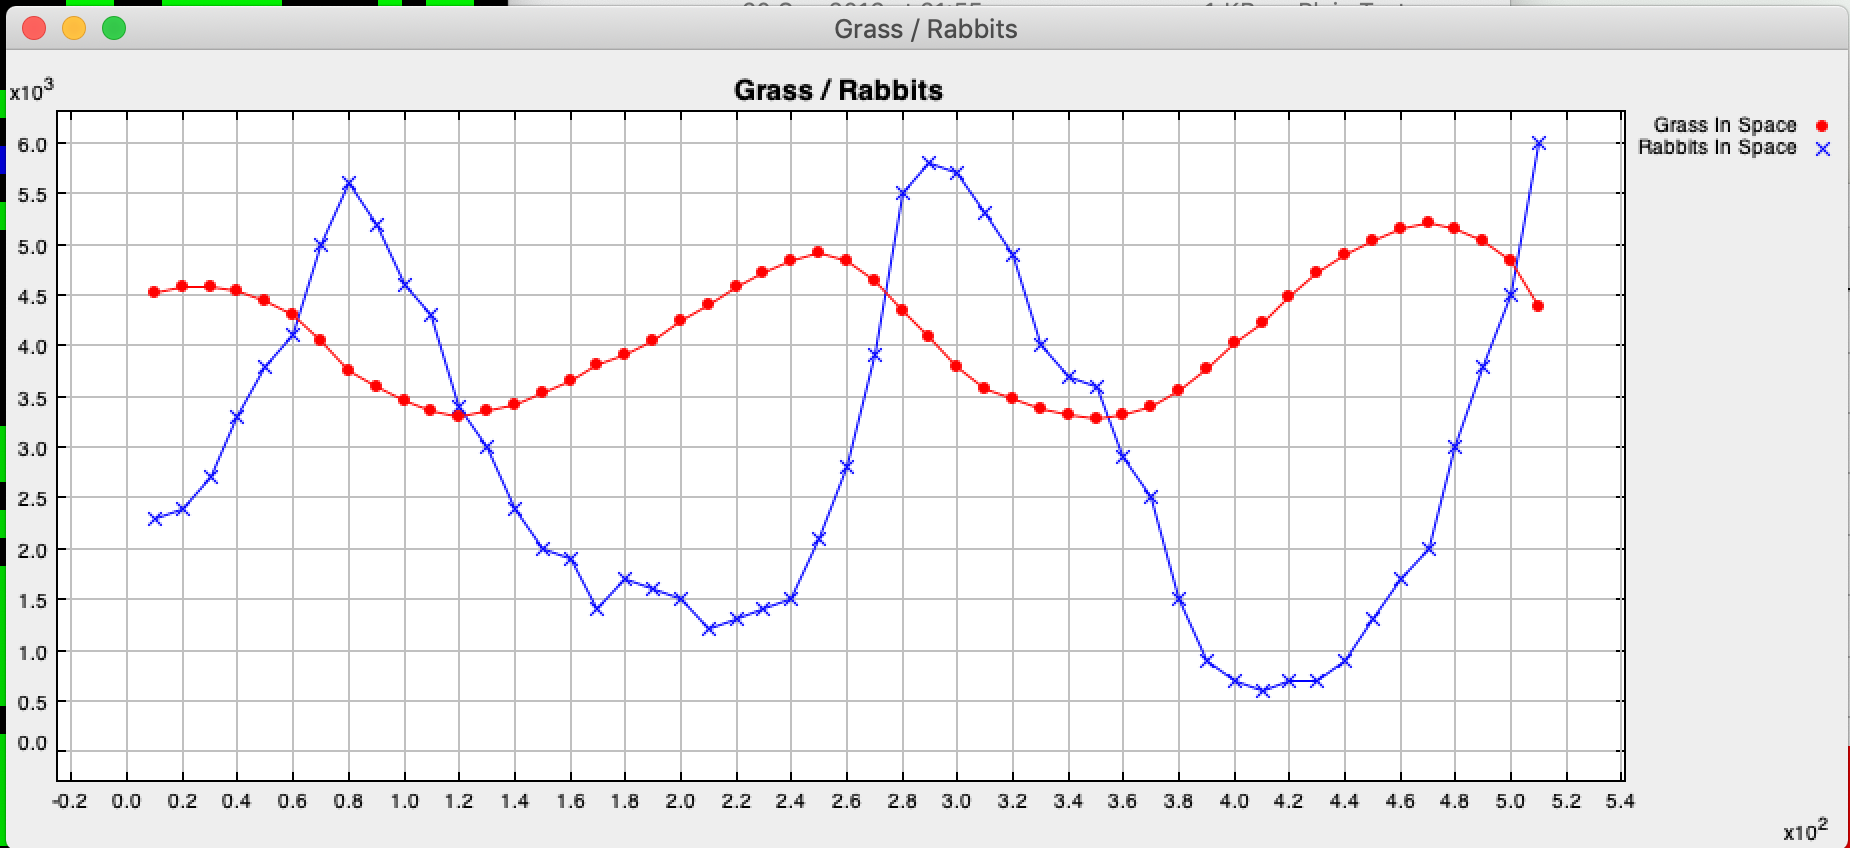
\includegraphics[width=1.0\textwidth]{ex1-chart-20}
\centering
\label{fig:ex1-20}
\caption{ 20 initial rabbits }
\end{figure}

\begin{figure}[H]
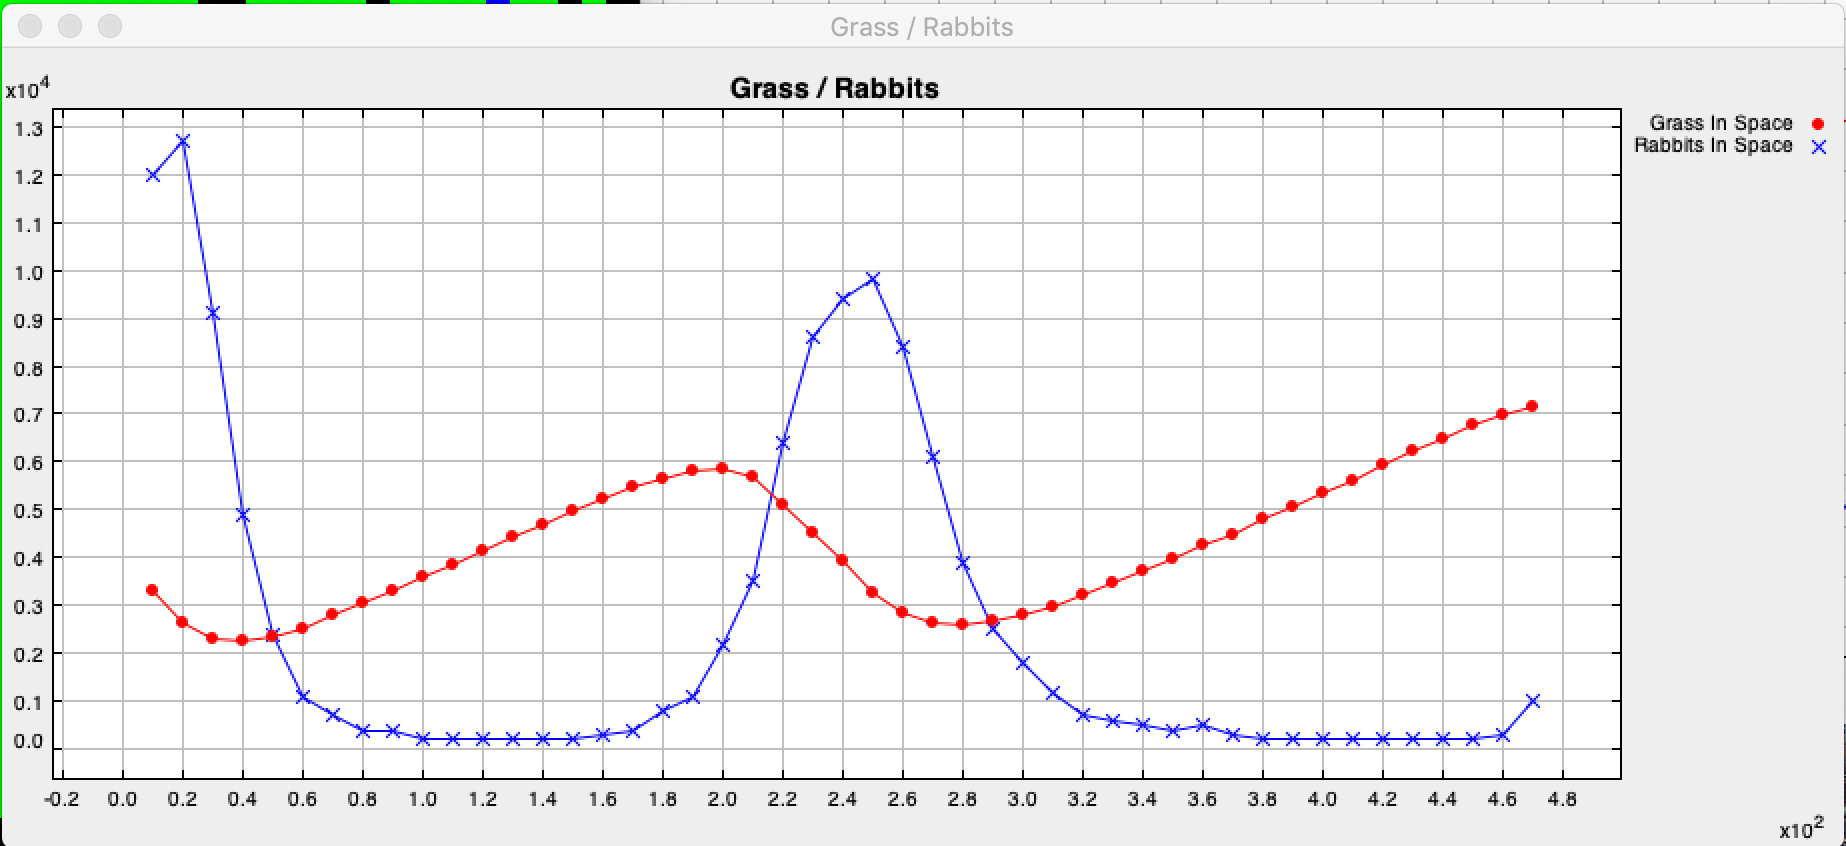
\includegraphics[width=1.0\textwidth]{ex1-chart-100}
\centering
\label{fig:ex1-100}
\caption{ 100 initial rabbits }
\end{figure}


\subsubsection{Setting}
\begin{figure}[H]
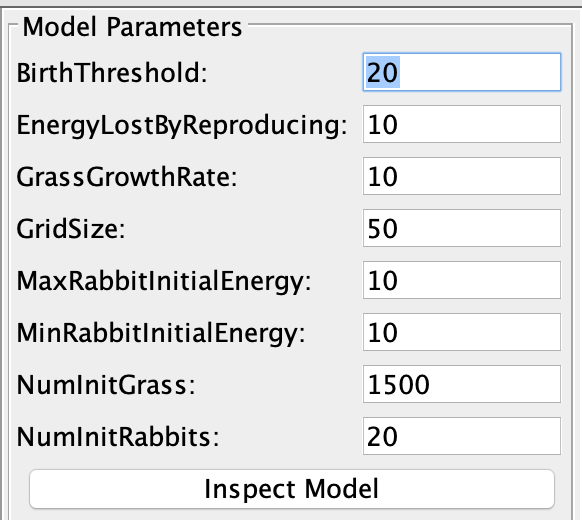
\includegraphics[width=0.5\textwidth]{ex1-params}
\centering
\label{fig:movement-directions}
\caption{ Ex 1 params }
\end{figure}


\subsubsection{Observations}
We can observe that variating the initial amount of rabbits does not impact the population on long term; there are still going to be periods of great decline in population (when food is going to drastically increase) followed by a population increase and the decrease of food resources.

\subsection{Experiment 2 ~ variating the energy lost through reproduction}

\begin{figure}[H]
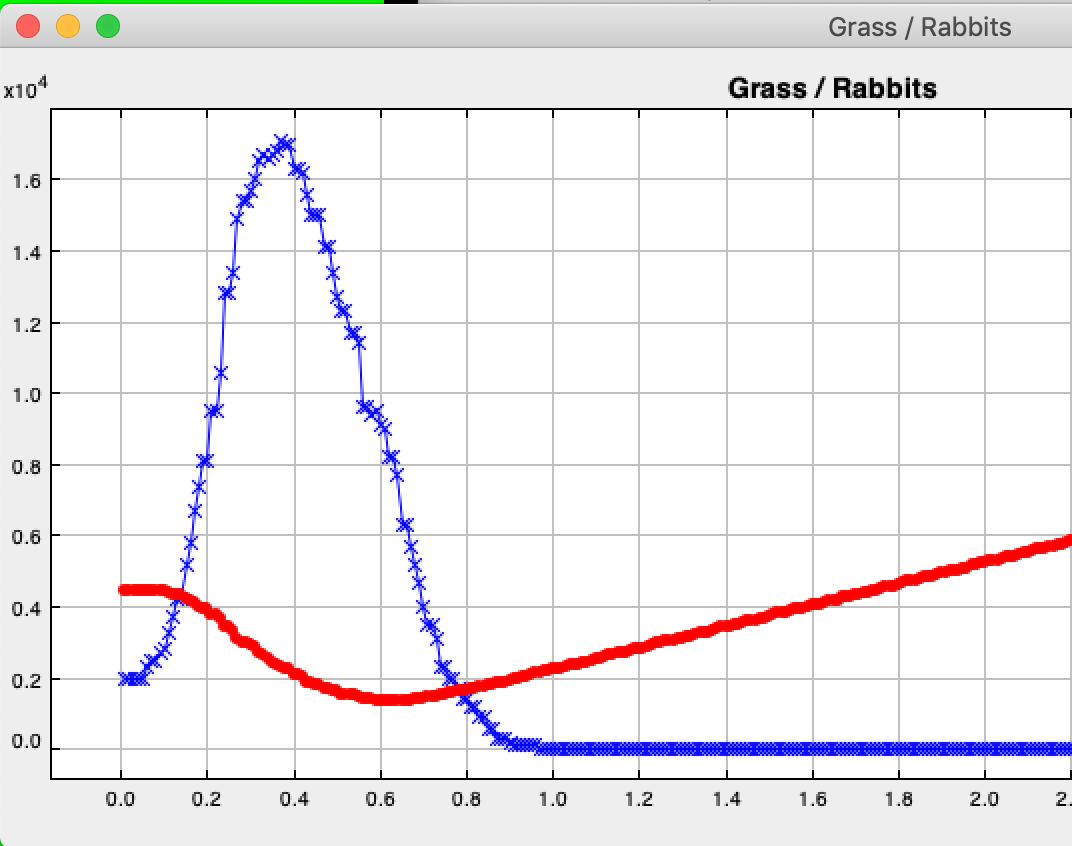
\includegraphics[width=0.8\textwidth]{ex2-chart-1}
\centering
\label{fig:ex2-1}
\caption{ cost of reproduction is 1 }
\end{figure}

\begin{figure}[H]
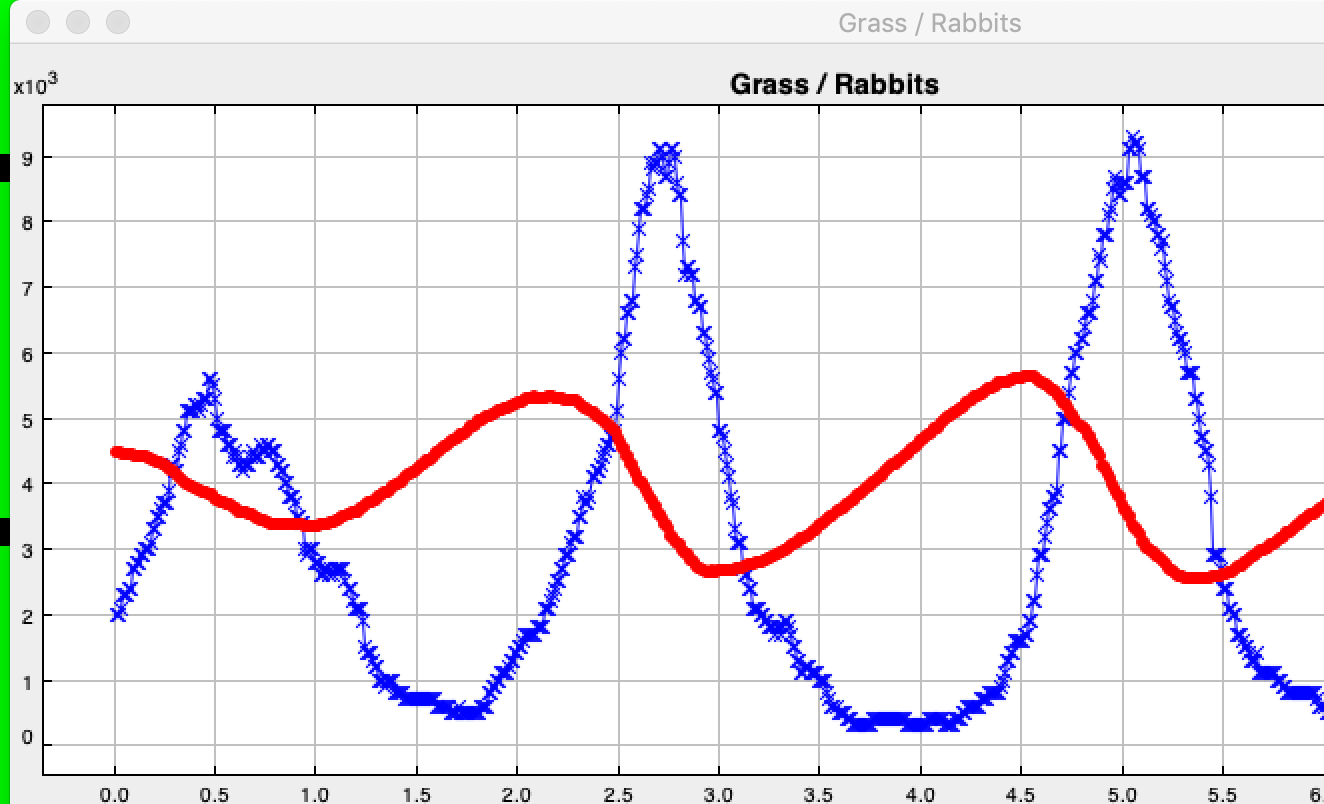
\includegraphics[width=0.8\textwidth]{ex2-chart-10}
\centering
\label{fig:ex2-10}
\caption{ cost of reproduction is 10 }
\end{figure}

\begin{figure}[H]
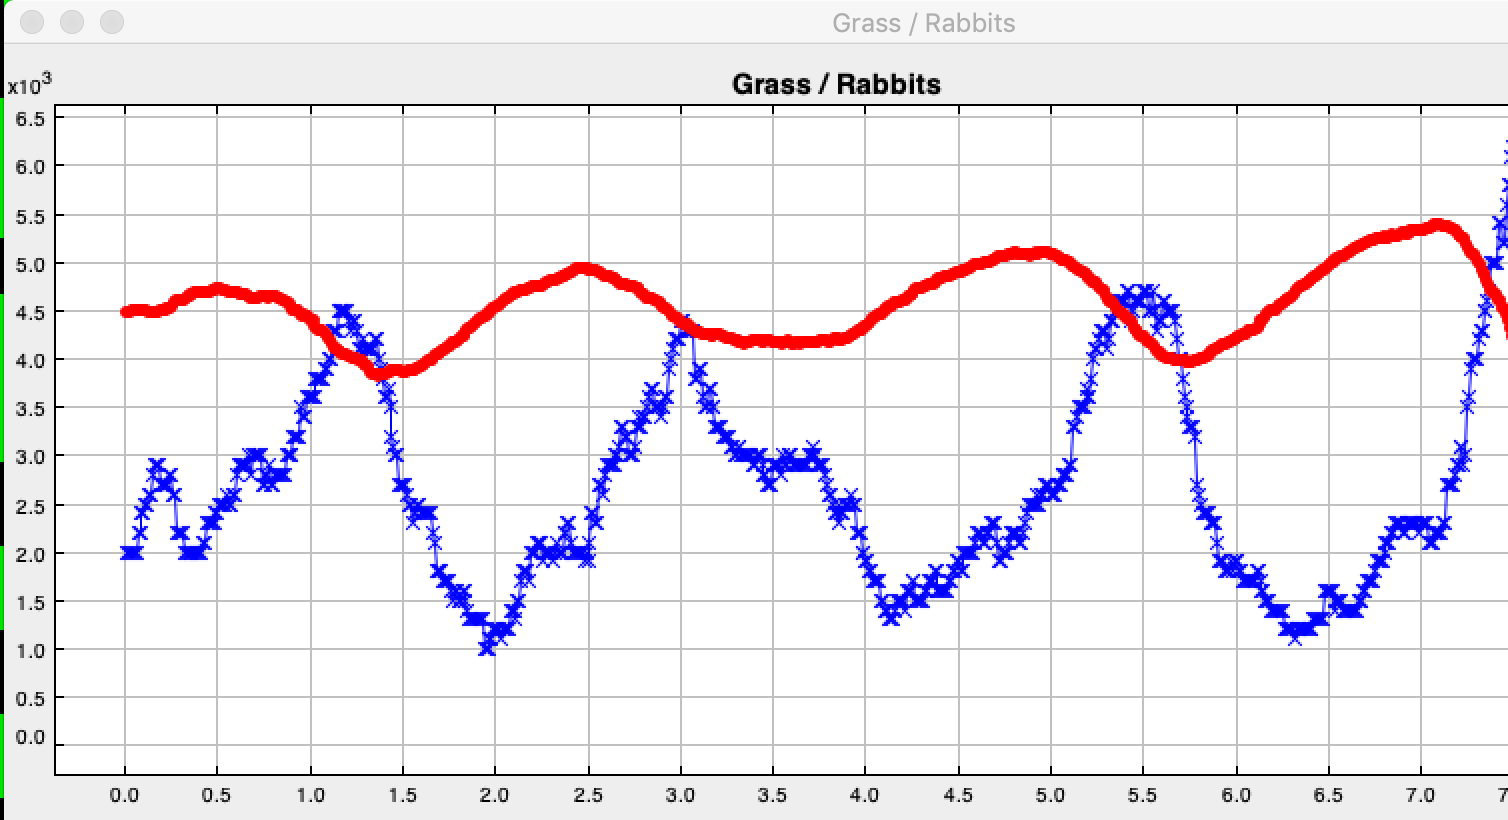
\includegraphics[width=0.8\textwidth]{ex2-chart-15}
\centering
\label{fig:ex2-15}
\caption{ cost of reproduction is 15 }
\end{figure}

\begin{figure}[H]
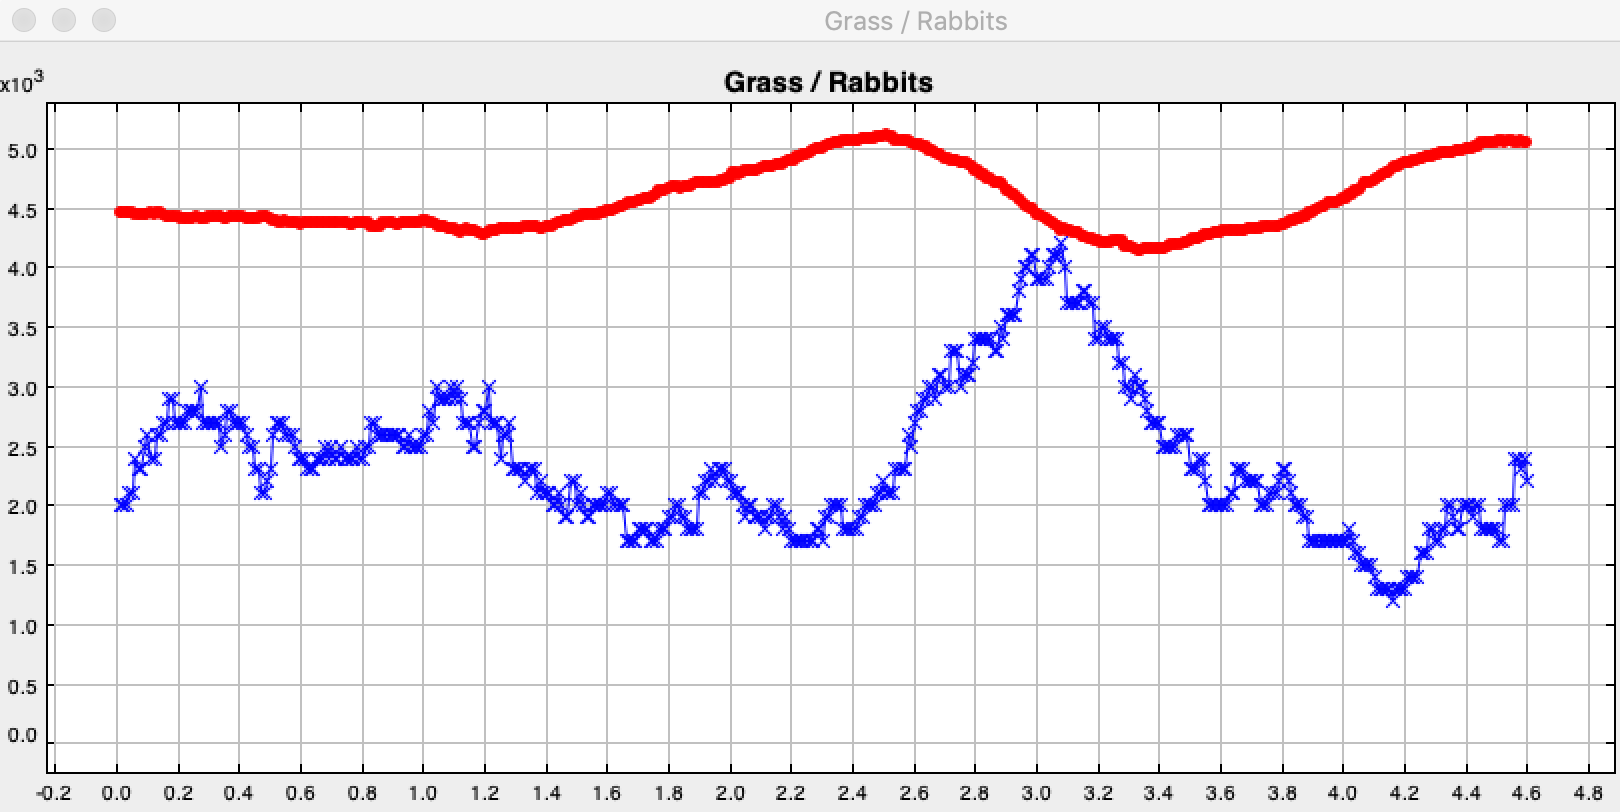
\includegraphics[width=0.8\textwidth]{ex2-chart-18}
\centering
\label{fig:ex2-18}
\caption{ cost of reproduction is 18 }
\end{figure}

\subsubsection{Setting}
\begin{figure}[H]
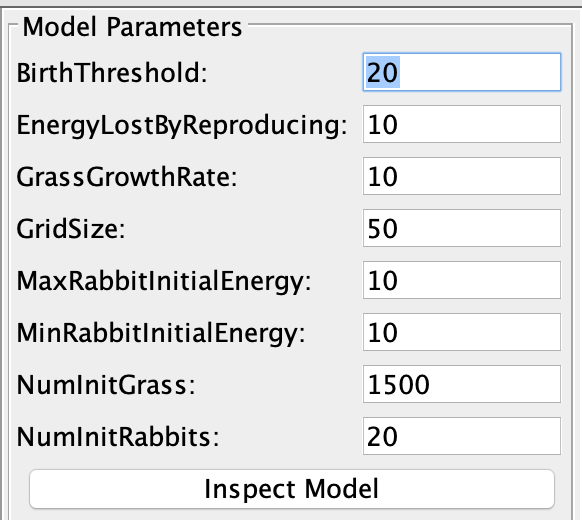
\includegraphics[width=0.5\textwidth]{ex1-params}
\centering
\label{fig:movement-directions}
\caption{ Ex 1 params }
\end{figure}

\subsubsection{Observations}
As the cost of reproduction increase the amount of available grass increases too.

The first simulation (the one with cost of reproduction 1) has an interesting results, as the rabbit population booms too fast it exhausts the available grass (not allowing enough time for more grass to grow) and this leads to extermination for rabbits.



\subsection{Variation in birth threshold}

\begin{figure}[H]
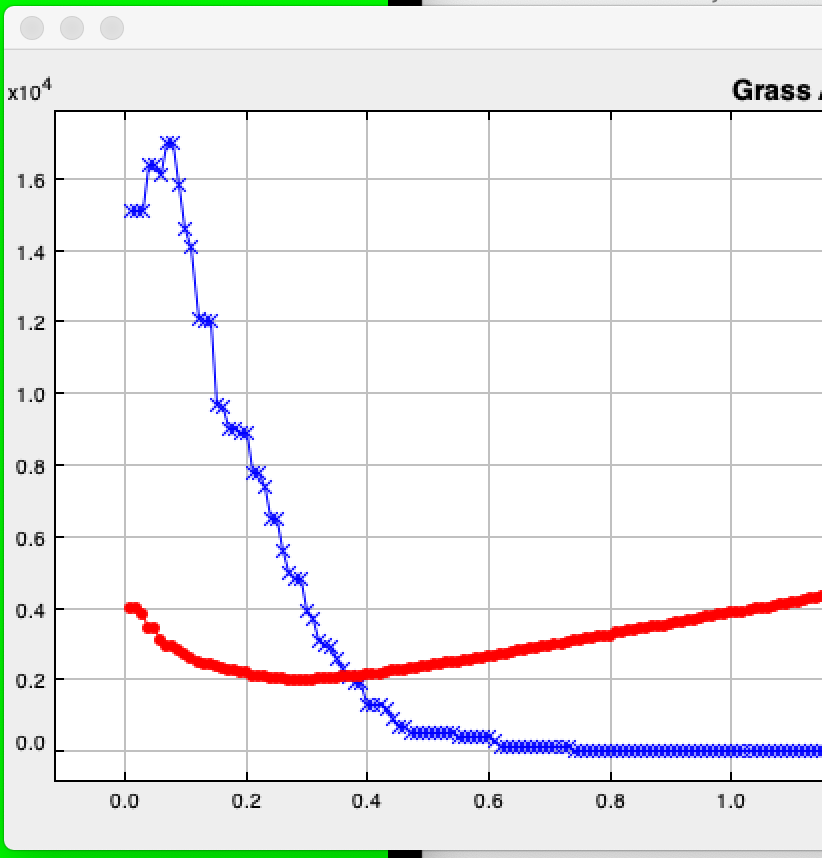
\includegraphics[width=0.5\textwidth]{ex3-chart-12}
\centering
\label{fig:ex3-12}
\caption{ birth threshold is 12 }
\end{figure}

\begin{figure}[H]
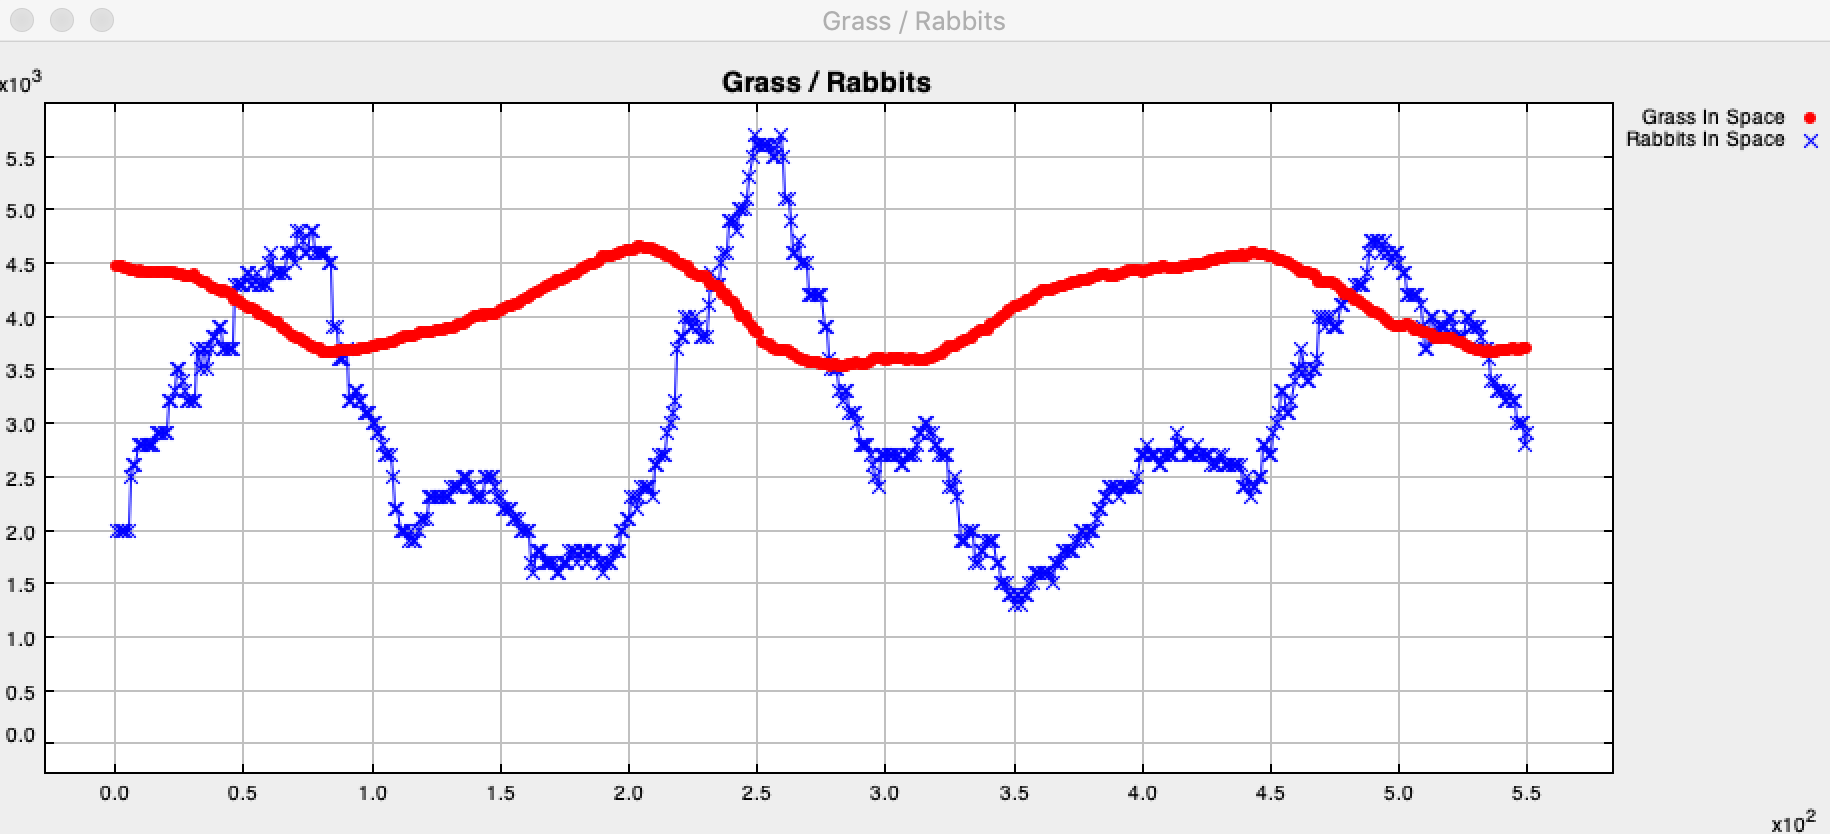
\includegraphics[width=0.8\textwidth]{ex3-chart-20}
\centering
\label{fig:ex3-20}
\caption{ birth threshold is 20 (~500 ticks) }
\end{figure}

\begin{figure}[H]
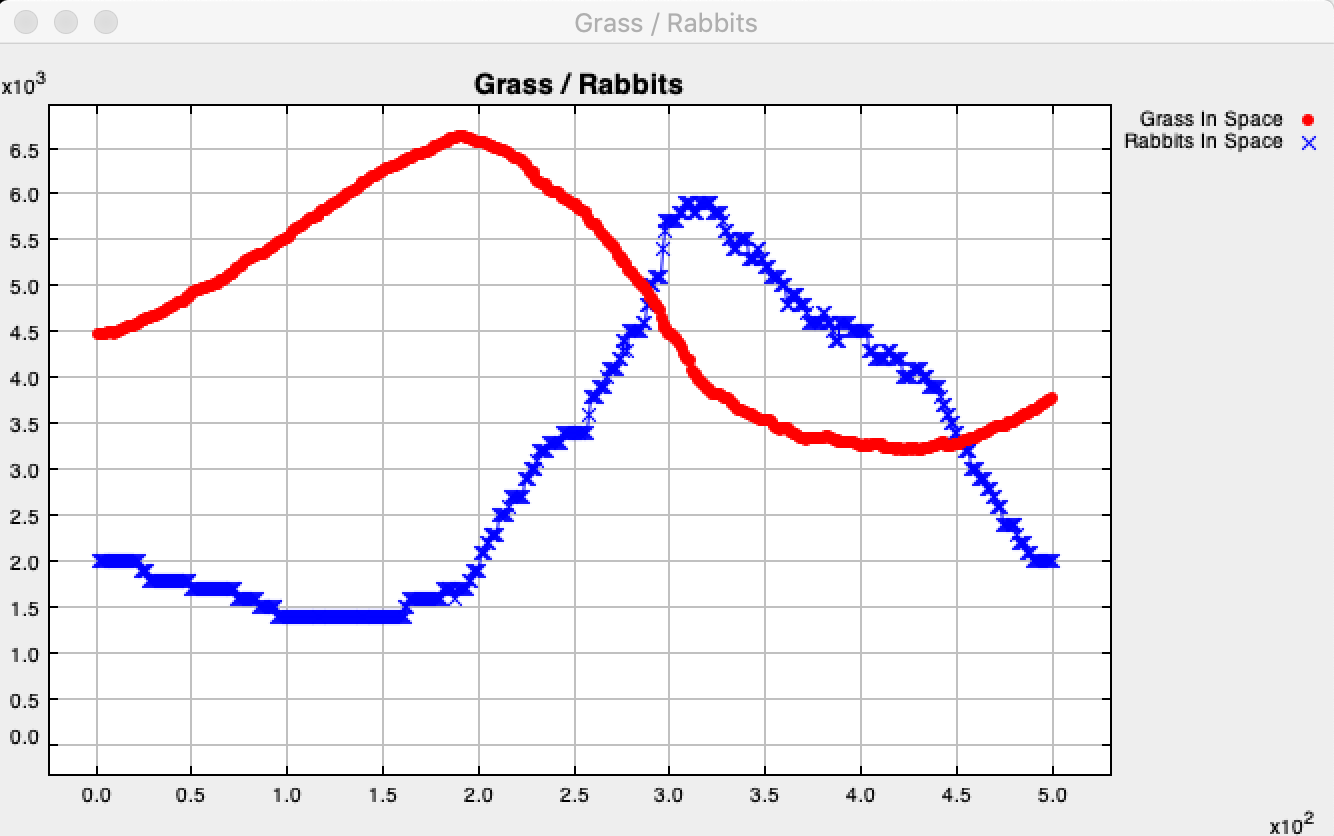
\includegraphics[width=0.8\textwidth]{ex3-chart-80}
\centering
\label{fig:ex3-80}
\caption{ birth threshold is 80 (~500 ticks) }
\end{figure}

\begin{figure}[H]
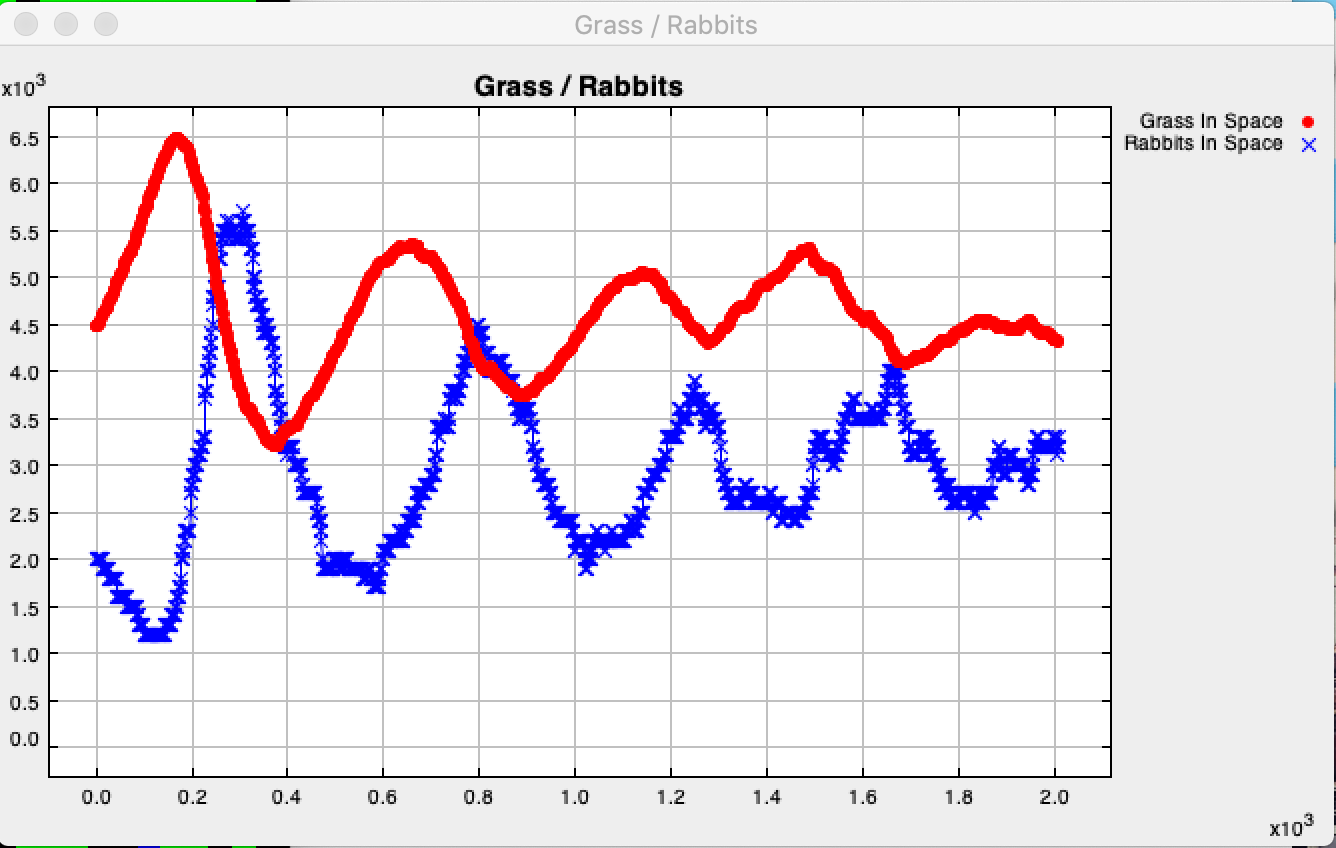
\includegraphics[width=0.8\textwidth]{ex3-chart-80-2000}
\centering
\label{fig:ex3-80-2000}
\caption{ birth threshold is 80 (~2000 ticks) }
\end{figure}


\subsubsection{Setting}
\begin{figure}[H]
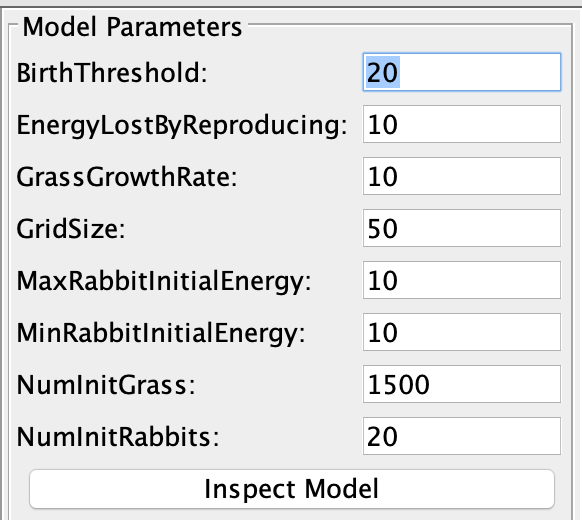
\includegraphics[width=0.5\textwidth]{ex1-params}
\centering
\label{fig:movement-directions}
\caption{ Ex 1 params }
\end{figure}

\subsubsection{Observations}
A birth threshold of 20 provides a right balance for the population to thrive (but not overpopulate).

The other represent the two extremes, the case of birth threshold being 12 (with an initial energy value of 10) leads to a fast overpopulation of rabbits that is going to cause their extinction; the threshold of 80 provides room for grass to grow until the rabbit population will catch up, in time this value provides the right balance
% Elaborate on the observed results %

\end{document}